\section{شرح پروژه}
در این پروژه ما یک سامانه‌ی 
\lr{iot}
رصد وضعیت هوا طراحی کردیم که وضعیت 3 نوع گاز سمی در هوا را اندازه‌‌گیری می‌کند و با توجه به مقادیر این گاز‌ها اخطار‌های لازم را به کاربران می‌دهد. این سامانه اطلاعات وضعیت هوا را از تعدادی دستگاه که هر یک سه سنسور مخصوص به گاز ‌دارند می‌گیرد و میانگین وضعیت آن‌ها را نشان می‌دهد و بر اساس وضعیت گاز با بیشترین غلظت وضعیت آلودگی کلی را نشان می‌دهد. این سامانه به صورت یک اپلیکیشن گوشی پیاده‌سازی شده است که با یک لوکیشن خاص کار می‌کند و همچنین یک وب‌سرور که اطلاعات میانگین چند دستگاه را نمایش می‌دهد. شمای کلی طراحی را در شکل زیر مشاهده می‌کنید. 
\begin{figure}[h!]
	\centering		
 	\includegraphics[width=\linewidth]{figs/iot.png}
	\caption{شمای کلی سیستم}
\end{figure}


\subsection{تغییرات نسبت به پروپوزال اولیه}
در پروپوزال پروژه ما سیستم را به صورت یک دستگاه در نظر گرفتیم اما در ارائه‌ی اولیه تصمیم بر آن شد که قابلیت داشتن دستگاه در چند لوکیشن مختلف را نیز پیاده‌سازی کنیم. بنابراین ما یک وب سرور طراحی کردیم که بتواند مقادیر گاز‌ها را از چند برد مختلف در لوکیشن‌های مختلف بگیرد و میانگین آن‌ها را گزارش دهد که مشابه کاری است که دستگاه‌های رصد هوای مزاکر مناطق مختلف شهر انجام می‌دهند. همچنین اپلیکیشن گوشی نیز طراحی کردیم که مطابق آنچه در پروپوزال گفته شده بود از یک دستگاه آمار را می‌گیرد و مشابه یک سامانه رصد هوای خانگی برای ساختمان‌های هوشمند عمل می‌کند.  

\section{طراحی و پیاده سازی}
- کلا iot builder و این داستانا رو یه ذره بگیم و نوع پروژه توی پرتئوس و اینا

در این پروژه ما با استفاده از 
\href{https://labcenter.s3.amazonaws.com/downloads/iotHelp.pdf}{iot-builder}
یک 
\subsection{شماتیک مدار}
شماتیک مدار را در شکل زیر مشاهده می‌کنید. در این مدار یک برد 
\lr{Arduino Yun}
که برای کاربرد‌های 
\lr{iot}
مناسب است و سه سنسور
\lr{LM35DZ}
تعبیه شده است که سنسور‌های دما هستند اما ما از آن‌ها به عنوان سنسور تشخیص گاز استفاده می‌کنیم. در پروپوزال ما سنسور‌های واقعی اندازه‌گیری گاز 
\lr{MQ-7}
و 
\lr{MQ-2}
و
\lr{MQ-135}
را استفاده کرده بودیم اما چون این سنسور‌ها در 
\lr{Proteus}
نبودند ما از سنسور‌های جایگزین اندازه‌گیری دما استفاده کردیم.
\begin{figure}[h!]
	\centering		
	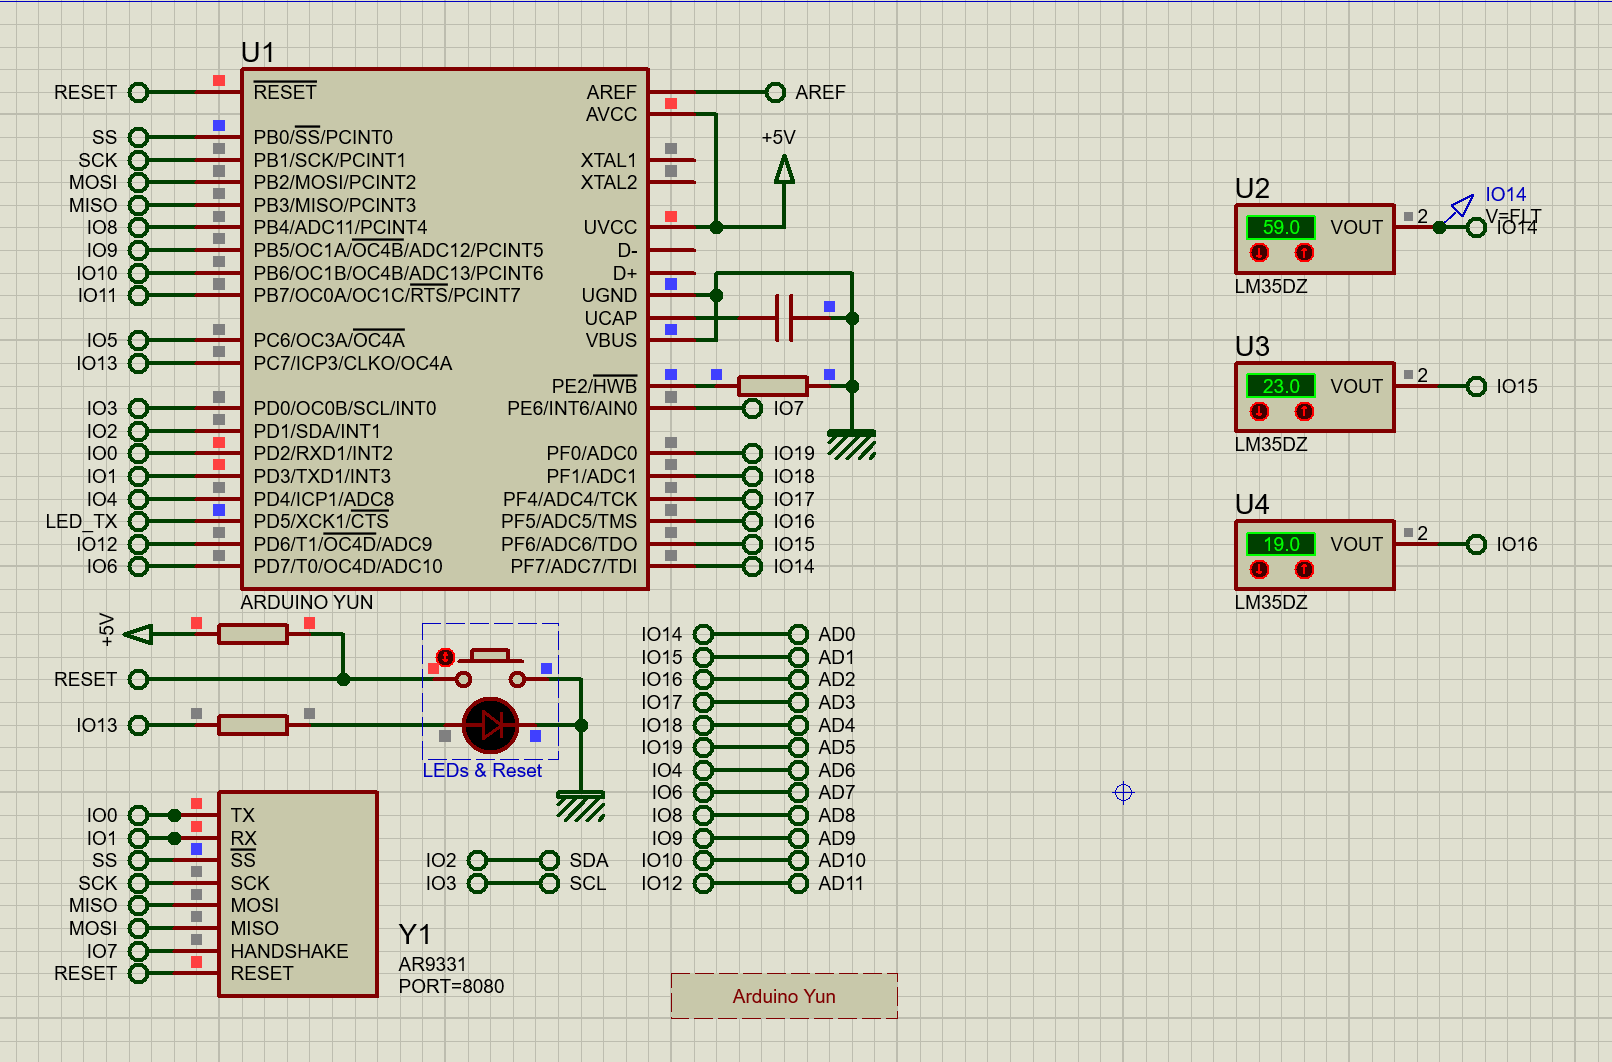
\includegraphics[width=\linewidth]{figs/circuit.png}
	\caption{شماتیک مدار}
\end{figure}

\subsection{توضیح کلی کد}
اینجا کلا توضیج میدیم که کد چه جوریه و سیستم چه جوریه و اینا

\subsection{اپلیکیشن گوشی}
برای طراحی اپلیکیشن گوشی ما از قابلیت‌های 
\lr{Visual Designer}
استفاده کردیم و کنترلر‌های 
\lr{iot}
زیر را 

- عکس از پنل گوشی

- توضیج این که چطوری از طریق وای فای با اضافه کردن ip دستگاه از روی گوشی ریزالتو می بینیم و اینا

\subsection{وب‌سرور و میانگین‌گیری از نتایج چند دستگاه}
- اینجا راجع به  
elastic search
 اینا توضیح میدیم و ساختن ایندکسو پوش کردن ریزالتا و ...

\section{فایل‌ها و شیوه ‌ی اجرای برنامه}
برای اجرای برنامه مراحل زیر را طی می‌کنیم:
\begin{itemize}
	\item 
	\textbf{راه اندازی سرور الستیک}:
	برای راه‌اندازی وب سرور باید  
	\lr{elasticsearch}
	روی سیستم نصب باشد. ورژن‌های مختلف نرم‌افزار در 
	\href{https://www.elastic.co/downloads/elasticsearch}{اینجا}
	موجود است. پس از دانلود و 
	\lr{unzip}
	کردن وارد پوشه می‌شویم فایل 
	\lr{elasticsearch.yml}
	را با فایلی که پوشه‌ی 
	\lr{config}
	از پروژه قرار دارد جایگزین می‌کنیم. این فایل قابلیت 
	\lr{cors}
	را به سرور اضافه می‌کند. 
	
	 سپس دستور 
\begin{latin}
\begin{lstlisting}[language=bash]
elasticsearch-7.8.0> .\bin\elasticsearch
\end{lstlisting}
\end{latin}
را می‌زنیم تا سرور راه بیفتد. در نهایت با دستور زیر فایل 
\lr{index.py}
را ران می‌کنیم.  
\begin{latin}
\begin{lstlisting}[language=bash]
python elasticsearch\index.py
\end{lstlisting}
\end{latin}
تا یک ایندکس خالی به نام 
\lr{iot}
در سرور الستیک ساخته شود (روی یک سیستم فقط یک بار نیاز است این دستور اجرا شود). 
	\item 
	\textbf{فایل‌های \lr{Arduino Yun}}:
	پس از باز کردن پروژه در پروتئوس پوشه‌ای با نامی مشابه زیر در آدرسی مشابه زیر ساخته می‌شود:
\begin{latin}
\begin{lstlisting}[language=bash]

\end{lstlisting}
\end{latin}	
در این پوشه یک پوشه‌ی دیگر به نام 
\lr{ARDUINO YUN}
قرار دارد که محتوای آن باید با محتوای این پوشه که ما در فایل‌های پروژه قرار دادیم جایگزین شود. 
		
	\item 
	\textbf{راه‌اندازی کلاینت گوشی همراه}:
	برای راه‌اندازی کلاینت گوشی همراه باید نرم‌افزار 
	\lr{IoT Controller}
	را از
	\href{https://play.google.com/store/apps/details?id=com.labcenter.iotbuilder&hl=en_GB}{اینجا}
	 نصب کنیم. سپس به صورت زیر در بخش 
	 \lr{Discover}
	 آی پی و پورتی که برد آردینو روی آن در حال اجرا است را وارد کنیم تا گوشی به برد وصل شود. 
	 \begin{figure}[h!]
	 	\centering			 	
	 	\subfloat{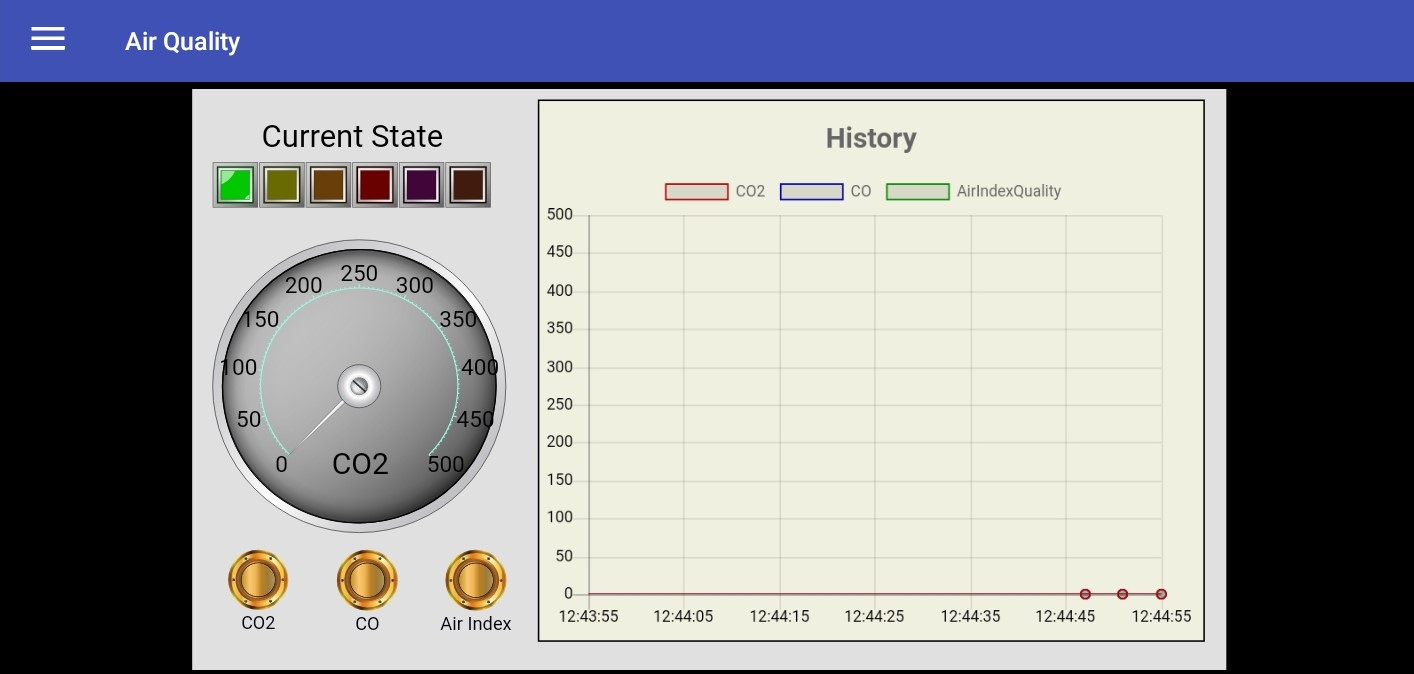
\includegraphics[width=0.45\textwidth]{figs/pic2.jpg}}
	 	\hfill	 	
	 	\subfloat{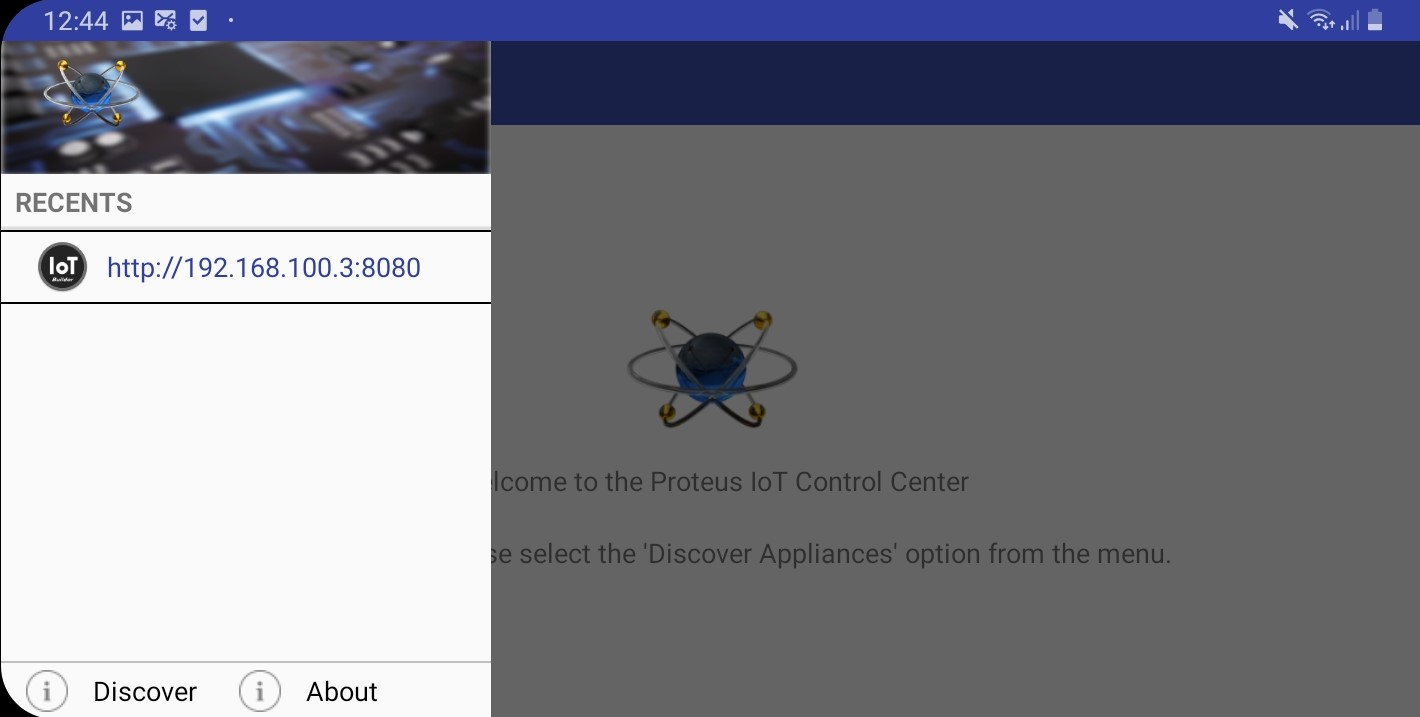
\includegraphics[width=0.42\textwidth]{figs/pic1.jpg}}
	 	\caption{شیوه‌ی اتصال گوشی به برد}	
	 \end{figure}
	
	\item
	\textbf{مشاهده نتایج در وب‌سرور}:
	برای مشاهده‌ی نتایج در وب‌سرور فایل 
	\lr{web.html}
	در پوشه‌ی 
	\lr{Web}
	را اجرا می‌کنیم. 	
\end{itemize}

\section{سیمولیشن و نتایج}
- یه تعدادی عکس از اجرای برنامه از روی گوشی با یه لوکیشن و از روی وب سرور با مثلا دو تا لوکیشن


\section{چالش‌ها}